\documentclass[russian,utf8,emptystyle,reduceheight=5mm]{eskdtext}

% packages
%
% Тестовое наполнение текстом
% При написании работы - удалить пакет и комманды \lipsum
\usepackage{lipsum}
%
\usepackage{eskdplain}
\usepackage{graphicx}
\usepackage{datetime}
\usepackage{enumitem} % for lists
\usepackage{ulem} % for underlining
\usepackage{lastpage} % Number of pages
\usepackage{hyperref} % Links in pdf

% setup
\newcommand{\FrontPageDepartment}{ЭМ} %Факультет
\newcommand{\FrontPageSubdepartment}{Менеджмента} %Кафедра
\newcommand{\WorkType}{Контрольная работа} %Тип работы (заголовок)
\newcommand{\Subject}{Предмет} %по ... родительный падеж
\newcommand{\Topic}{Тема контрольной работы} %Тема
\newcommand{\Professor}{Иванов~И.~И.} %Руководитель
\newcommand{\Student}{Петров~П.~П.} %Студент
\newcommand{\Group}{ИСм-112} %Группа
\newcommand{\FrontPageDate}{\ddmmyyyydate\today} %Дата

\ESKDsignature{МИВУ 230400.68 ПЗ} % Код специальности и тип работы

% eskdx setup
\ESKDletter{}{У}{}
\ESKDtitle{\Topic}
\ESKDchecker{\Professor}
\ESKDauthor{\Student}
\ESKDcolumnIX{МИ ВлГУ\\ \Group}

\addto\captionsrussian{\def\refname{Список использованных источников}}
\sloppy % split long lines

% graphics path
\graphicspath{{src/img/}}


% verbatim setup
\newcommand{\verbatimFont}{
\fontsize{10pt}{12pt}\selectfont
\baselineskip=1em
}


% workaround for regression in babel package on linux
\providecommand{\No}{\textnumero}


% remove vertical space from lists
\renewcommand{\alph}[1]{\asbuk{#1}} % костыль для кирилической нумерации вместо латинской
\setlist{nolistsep} % убираем дополнительные вертикальные отступы вокруг списков
\setenumerate[1]{label=\alph*), fullwidth, itemindent=\parindent,  listparindent=\parindent}
\setenumerate[2]{label=\arabic*), fullwidth, itemindent=\parindent, listparindent=\parindent, leftmargin=\parindent}
\setitemize{fullwidth, itemindent=\parindent, listparindent=\parindent}
\newlength{\PAGEborderLR}
\newlength{\PAGEborderTB}

\setlength{\PAGEborderLR}{2cm}
\setlength{\PAGEborderTB}{2cm}

% Set up page
\setlength{\hoffset}{-2.54cm + \PAGEborderLR}
\setlength{\voffset}{-2.54cm + \PAGEborderTB}
\setlength{\topskip}{0pt}
\setlength{\footskip}{21pt}
\setlength{\oddsidemargin}{0pt}
\setlength{\evensidemargin}{0pt}
\setlength{\topmargin}{0pt}
\setlength{\headheight}{0pt}
\setlength{\headsep}{0pt}
\setlength{\textwidth}{210mm-\PAGEborderLR*2}
\setlength{\textheight}{297mm-\PAGEborderTB*2-\footskip}
\setlength{\marginparsep}{0pt}
\setlength{\marginparwidth}{0pt}
\setlength{\marginparpush}{0pt}

% main document
\begin{document}
% Титул
\ESKDthisStyle{empty}
\setlength{\topskip}{15pt}
\newlength{\frontpagefk} % Ширина поля Факультет/Кафедра
\setlength{\frontpagefk}{6cm}
\newlength{\frontpagerb} % Ширина надписей Руководитель/Студент и пр. под темой
\setlength{\frontpagerb}{6cm}
\newlength{\frontpagerbspace} % ??? (do not remove)
\setlength{\frontpagerbspace}{1cm}
\newlength{\FrontPageSubjSpace} % Ширина пробела до и после названия предмета
\setlength{\FrontPageSubjSpace}{1cm}
\newlength{\FrontPageTopicSpace} % Ширина пробела до и после темы
\setlength{\FrontPageTopicSpace}{0.5cm}

\thispagestyle{empty}
\begin{center}
{
\vspace*{-1.5cm}
\baselineskip=1.3em
{\small Министерство образования и науки Российской Федерации}\\
\textbf{Муромский институт (филиал)}\\
{\footnotesize федерального государственного бюджетного образовательного учреждения\\
высшего профессионального образования}\\
\textbf{<<Владимирский государственный университет\\
имени Александра Григорьевича и Николая Григорьевича\\
Столетовых>>\\
(МИ (филиал) ВлГУ)\\}
}

\bigskip
\begin{tabular}{l c}
\textbf{Факультет}&\underline{\makebox[\frontpagefk]{\FrontPageDepartment}}\\
\textbf{Кафедра}&\underline{\makebox[\frontpagefk]{\FrontPageSubdepartment}}\\
\end{tabular}

\vspace{\fill}
\begin{Huge}
\textbf{\textsl{\WorkType}}
\end{Huge}

\vspace{\fill}
по \underline{\makebox[\FrontPageSubjSpace]{}\Subject\makebox[\FrontPageSubjSpace]{}}

\smallskip
\parbox{15cm}{\centering{Тема: \uline{\makebox[\FrontPageTopicSpace]{}\Topic\makebox[\FrontPageTopicSpace]{}}}}

\vspace{\fill}

\begin{flushright}
\makebox[\frontpagerb][c]{
\makebox[\frontpagerb][l]{Руководитель}\hspace{\frontpagerbspace}}

\smallskip
\makebox[\frontpagerb][c]{
\raisebox{-\baselineskip}{\shortstack{\underline{\makebox[\frontpagerb][l]{\Professor}}\\
\begin{footnotesize}
(фамилия, инициалы)
\end{footnotesize}}}\hspace{\frontpagerbspace}}

\bigskip
\makebox[\frontpagerb][c]{
\raisebox{-\baselineskip}{\shortstack{\underline{\makebox[\frontpagerb][l]{}}\\
\begin{footnotesize}
(подпись)\hfill(дата)
\end{footnotesize}}}\hspace{\frontpagerbspace}}

\newcommand{\frontpagerbstudent}[2]{ %
\makebox[\frontpagerb]{ %
\raisebox{-\baselineskip}{\shortstack{#1\ \underline{\makebox[\frontpagerb-\widthof{#1\ }][c]{#2}}\\
\begin{footnotesize}
\makebox[\widthof{#1\ }][c]{}\makebox[\frontpagerb-\widthof{#1\ }][c]{(группа)}
\end{footnotesize}}}\hspace{\frontpagerbspace}}
}

\bigskip
\makebox[\frontpagerb][c]{\frontpagerbstudent{Студент}{\Group}}

\smallskip
\makebox[\frontpagerb][c]{
\raisebox{-\baselineskip}{\shortstack{\underline{\makebox[\frontpagerb][l]{\Student}}\\
\begin{footnotesize}
(фамилия, инициалы)
\end{footnotesize}}}\hspace{\frontpagerbspace}}

\renewcommand{\dateseparator}{.}

\bigskip
\makebox[\frontpagerb][c]{
\raisebox{-\baselineskip}{\shortstack{\underline{\makebox[\frontpagerb][r]{\FrontPageDate}}\\
\begin{footnotesize}
(подпись)\hfill(дата)
\end{footnotesize}}}\hspace{\frontpagerbspace}}

\end{flushright}

\vspace{\fill}
Муром \the\year
\vspace*{-1cm}
\end{center}
\setlength{\topskip}{0pt}
\newpage

% Аннотация
\ESKDthisStyle{empty}
\vspace*{\fill}
Курсовой проект посвящен разработке и реализации ...

В курсовом проекте подробно описано техническое задание, проведена разработка алгоритмов, программы, написано руководство, осуществлено тестирование системы.

Объём пояснительной записки составляет \pageref{LastPage} листов. Количество рисунков - 2 штуки. Таблицы отсутствуют.
\vspace*{\fill}
\newpage

% Содержание
\setcounter{page}{4}
\tableofcontents
\newpage

% Основной текст
\begin{center}
{\WorkType}
\\
Тема: {\Topic}
\\
Цель: Создание простейшей программы на языке Python с использованием QtQML. 
\end{center}
Задание:
Создание калькулятора.

Ход выполнения:
\begin{center}
Программа:
\end{center}
\begingroup
\fontsize{12pt}{12pt}\selectfont
\begin{verbatim}
from PyQt5.QtGui import QGuiApplication
from PyQt5.QtQml import QQmlApplicationEngine
from PyQt5.QtCore import QObject, pyqtSignal, pyqtSlot

class Calculator(QObject):
first_operand = ''
seond_operand = ''
g=False
def __init__(self):
QObject.__init__(self)

sumResult = pyqtSignal(float, arguments=['sum'])

subResult = pyqtSignal(float, arguments=['sub'])

clear=pyqtSignal(arguments=['C'])

@pyqtSlot()
def is_first(self):
return True

@pyqtSlot()
def clear(self):
self.first_operand=0.0 
self.g=False

@pyqtSlot(float,str)
def sub(self,c,sign):

self.sign=sign

if self.g==False:
self.first_operand = c
self.g=True
else:

self.sumResult.emit(self.first_operand - c)

@pyqtSlot(float,str)
def sum(self,c,sign):

self.sign=sign
if self.g==False:
self.first_operand = c
self.g=True
else:

self.sumResult.emit(self.first_operand + c)

@pyqtSlot(float,str)
def unmoj(self,c,sign):

self.sign=sign
if self.g==False:
self.first_operand = c
self.g=True
else:

self.sumResult.emit(self.first_operand * c)

@pyqtSlot(float,str)
def delen(self,c,sign):

self.sign=sign
if self.g==False:
self.first_operand = c
self.g=True
else:

self.sumResult.emit(self.first_operand / c)

@pyqtSlot(float)
def ravno(self,c):

if self.sign == "-":
a=self.first_operand - c
self.sumResult.emit(a)

self.first_operand=a 
elif self.sign == "+":
a=self.first_operand + c
self.sumResult.emit(a)

self.first_operand=a 
elif self.sign == "*":
a=self.first_operand * c
self.sumResult.emit(a)

self.first_operand=a 
elif self.sign == "/":
a=self.first_operand / c
self.sumResult.emit(a)

self.first_operand=a   

if __name__ == "__main__":
import sys

app = QGuiApplication(sys.argv)

engine = QQmlApplicationEngine()

calculator = Calculator()

engine.rootContext().setContextProperty("calculator", calculator)

engine.load("main.qml")

engine.quit.connect(app.quit)
sys.exit(app.exec_())


import QtQuick 2.5
import QtQuick.Controls 1.4
import QtQuick.Layouts 1.2

ApplicationWindow {
visible: true
width: 280
height: 300
title: qsTr("Калькулятор")
color: "whitesmoke"

// Input field of the first number
TextField {
id: sumResult
width: 260; 
height: 30;
x:10
y:10
}

Button {
text: qsTr ("0")
height: 40;
width: 50		   
x:10
y:50   

onClicked:{
sumResult.text+=("0")
}
}

Button {
text: qsTr ("1")
height: 40;
width: 50		   
x:80
y:50

onClicked:{
sumResult.text+=("1")
}
}

Button {
text: qsTr ("2")
height: 40;
width: 50		   
x:150
y:50

onClicked:{
sumResult.text+=("2")

}
}
Button {
text: qsTr ("3")
height: 40;
width: 50		   
x:10
y:100

onClicked:{
sumResult.text+=("3")
}
}
Button {
text: qsTr ("4")
height: 40;
width: 50		   
x:80
y:100

onClicked:{
sumResult.text+=("4")
}
}

Button {
text: qsTr ("5")
height: 40;
width: 50		   
x:150
y:100

onClicked:{
sumResult.text+=("5")
}
}
Button {
text: qsTr ("6")
height: 40;
width: 50		   
x:10
y:150

onClicked:{
sumResult.text+=("6")
}
}
Button {
text: qsTr ("7")
height: 40;
width: 50		   
x:80
y:150

onClicked:{
sumResult.text+=("7")
}
}
Button {
text: qsTr ("8")
height: 40;
width: 50		   
x:150
y:150

onClicked:{
sumResult.text+=("8")
}
}
Button {
text: qsTr ("9")
height: 40;
width: 50		   
x:10
y:200

onClicked:{
sumResult.text+=("9")
}
}
Button {
text: qsTr ("+")
height: 40;
width: 50		   
x:80
y:200
id: plus
onClicked:{

calculator.sum(sumResult.text,"+")
sumResult.text=("")
plus.enabled=false
min.enabled=false
umn.enabled=false
del.enabled=false
}
}
Button {
text: qsTr ("-")
height: 40;
width: 50		   
x:150
y:200
id: min 
onClicked:{
calculator.sub(sumResult.text,"-")
sumResult.text=("")
plus.enabled=false
min.enabled=false
umn.enabled=false
del.enabled=false
}
}
Button {
text: qsTr ("*")
height: 40;
width: 50		   
x:220
y:200
id: umn
onClicked:{

calculator.unmoj(sumResult.text,"*")
sumResult.text=("")
plus.enabled=false
min.enabled=false
umn.enabled=false
del.enabled=false
}
}
Button {
text: qsTr ("/")
height: 40;
width: 50		   
x:220
y:150
id: del
onClicked:{

calculator.delen(sumResult.text,"/")
sumResult.text=("")
plus.enabled=false
min.enabled=false
umn.enabled=false
del.enabled=false
}
}

Button {
text: qsTr ("CE")
height: 90;
width: 50		   
x:220
y:50

onClicked:{
calculator.clear()
sumResult.text=("")
}
}
Button {
text: qsTr ("=")
height: 40;
width: 260		   
x:10
y:250

onClicked:{

calculator.ravno(sumResult.text)
plus.enabled=true
min.enabled=true
umn.enabled=true
del.enabled=true
}		
}
Connections {
target: calculator

// Sum signal handler
onSumResult: {
// sum was set through arguments=['sum']
sumResult.text = sum
}

// Subtraction signal handler
onSubResult: {
// sub was set through arguments=['sub']
subResult.text = sub	  
}
}
}
\end{verbatim}
\endgroup
Изображен код программы калькулятор.
\begin{center}
Результат работы программы:
\end{center}

\begin{figure}[h]
	\centering
	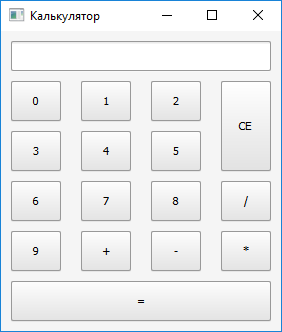
\includegraphics[scale=1]{s1}

	\label{fig:s1}
\end{figure}
Изображен результат работы программы.

Вывод: Создал простейшию программу на языке Python с использованием QtQML. 




\newpage

% Список литературы
\begin{thebibliography}{00}

\bibitem{bib_name1} источник 1

\bibitem{bib_name2} источник 2

\bibitem{bib_name3} источник 3

\bibitem{wiki_main} Википедия: свободная энциклопедия: на русском языке [Электронный ресурс] // URL:  http://ru.wikipedia.org/wiki/Заглавная\_страница  (дата обращения: 06.05.2013)

\bibitem{wiki_main} Википедия: свободная энциклопедия: на русском языке [Электронный ресурс] // URL:  http://ru.wikipedia.org/wiki/Заглавная\_страница  (дата обращения: \ddmmyyyydate\today)

\end{thebibliography}
\end{document}